\section{Ejercicio 3 - Implementación de módulos en verilog}
A continuación, se implementarán los circuitos pedidos en lenguaje verilog, comentando como fue su desarrollo e emplementación.
\subsection{DEMUX de 4 salidas}

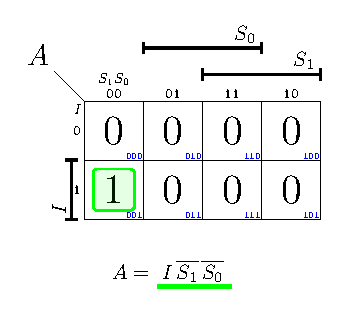
\includepdf{Ejercicio_3/Karnaugh/DEMUX/Salida_A.pdf}
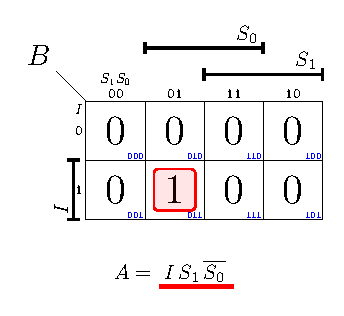
\includepdf{Ejercicio_3/Karnaugh/DEMUX/Salida_B.pdf}
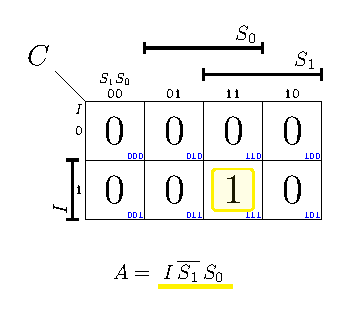
\includepdf{Ejercicio_3/Karnaugh/DEMUX/Salida_C.pdf}
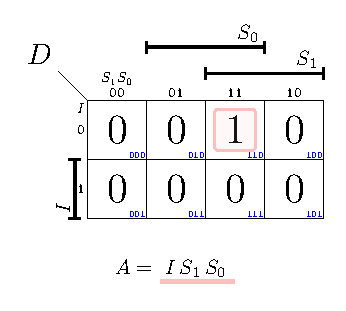
\includepdf{Ejercicio_3/Karnaugh/DEMUX/Salida_D.pdf}

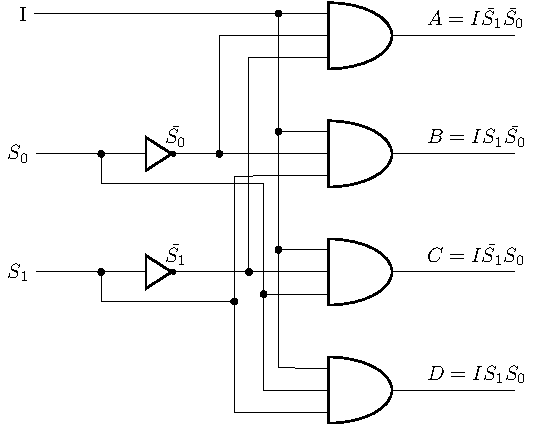
\includepdf{Ejercicio_3/Circuitos/Circuito_DEMUX.pdf}

\begin{table}[H]
	\begin{center}
		\begin{tabular}{ccc||cccc}

			$D$ &	$C_1$ &	$C_0$ &	$O_3$ & $O_2$ & $O_1$ &$O_0$ \\
			\hline
            0 & 0 & 0 & 0 & 0 & 0 & 0 \\
            
            0 & 0 & 1 & 0 & 0 & 0 & 0 \\
            
            0 & 1 & 0 & 0 & 0 & 0 & 0 \\
            
            0 & 1 & 1 & 0 & 0 & 0 & 0 \\
            
            1 & 0 & 0 & 1 & 0 & 0 & 0 \\
            
            1 & 0 & 1 & 0 & 1 & 0 & 0 \\
            
            1 & 1 & 0 & 0 & 0 & 1 & 0 \\
            
            1 & 1 & 1 & 0 & 0 & 0 & 1\\
			
		\end{tabular}
	\end{center}
\end{table}

\subsection{ENCODER de 4 entradas}

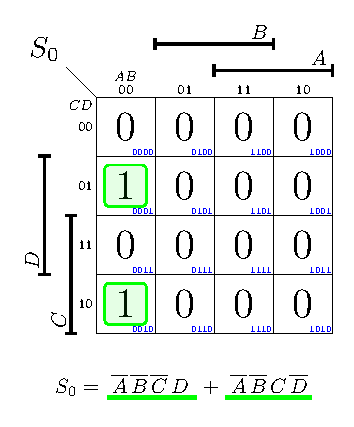
\includepdf{Ejercicio_3/Karnaugh/ENCODER/Salida_S_0.pdf}
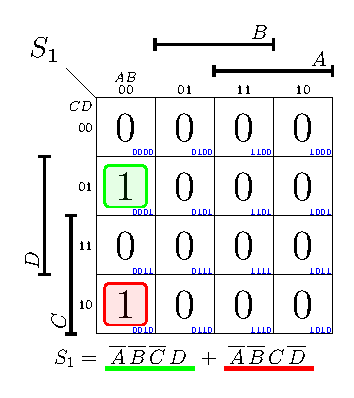
\includepdf{Ejercicio_3/Karnaugh/ENCODER/Salida_S_1.pdf}

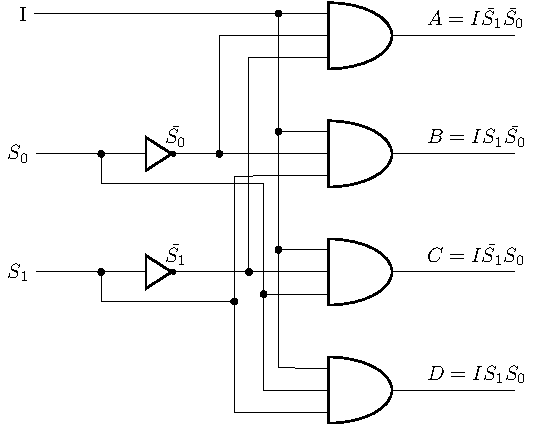
\includepdf{Ejercicio_3/Circuitos/Circuito_DEMUX.pdf}

\begin{table}[H]
	\begin{center}
		\begin{tabular}{c c c c||c c}

			$D$ &	$C$ &	$B$ &	$A$ & $S_1$ & $S_0$ \\
			\hline
            0 & 0 & 0 & 0 & 0 & 0   \\

            0 & 0 & 0 & 1 & 0 & 0   \\
  
            0 & 0 & 1 & 0 & 0 & 1   \\
          
            0 & 0 & 1 & 1 & 0 & 0   \\
         
            0 & 1 & 0 & 0 & 1 & 0   \\
           
            0 & 1 & 0 & 1 & 0 & 0   \\
         
            0 & 1 & 1 & 0 & 0 & 0   \\
        
            0 & 1 & 1 & 1 & 0 & 0   \\
         
            1 & 0 & 0 & 0 & 1 & 1   \\
        
            1 & 0 & 0 & 1 & 0 & 0   \\
         
            1 & 0 & 1 & 0 & 0 & 0   \\
       
            1 & 0 & 1 & 1 & 0 & 0  \\
          
            1 & 1 & 0 & 0 & 0 & 0   \\
      
            1 & 1 & 0 & 1 & 0 & 0   \\
        
            1 & 1 & 1 & 0 & 0 & 0   \\
          
            1 & 1 & 1 & 1 & 0 & 0  \\
		
		\end{tabular}
	\end{center}
\end{table}